\documentclass[12pt,a4paper]{article}
\usepackage{amsmath,amssymb,amsthm,epsf, graphicx, rotating}
\usepackage{fancyhdr}
\graphicspath{ {./images/} }

\pagestyle{empty}
\setlength{\parindent}{0pt}
\setlength{\textwidth}{6.5in}
\setlength{\oddsidemargin}{0in}
\addtolength{\textheight}{1in}

\renewcommand\theenumi{\alph{enumi}}
\renewcommand\labelenumi{(\theenumi)}

\newcommand{\Z}{\mathbb{Z}}
\newcommand{\F}{\mathbb{F}}
\newcommand{\R}{\mathbb{R}}
\newcommand{\C}{\mathbb{C}}
\newcommand{\N}{\mathbb{N}}
\renewcommand\vec{\mathbf}

\pagestyle{fancy}
\fancyhf{}
\fancyhead[LE, RO]{Ryan Liu}

\theoremstyle{definition}
\newtheorem{problem}{}

\author{Ryan Liu}
\title{MATH 442 Homework 2}
\begin{document}

\begin{center}
{\huge MATH 442 \par}
{\Large Homework  2  \par}
{\normalsize Name: Ryan Zhuo Lun Liu \par}
{\normalsize Student Number: 30328141 \par}
{\normalsize Collaborators: Jagjot Jhajj and Robert Benjamin Lang }
\end{center}

\begin{problem}
The local council in K\"onigsberg eventually decide to demolish one bridge. Does there exist  a bridge they can demolish so the citizens can find a route through the town crossing each bridge only once and \emph{not} finish up where they started? Explain your answer. \\

\underline{Answer:} \\
\centerline{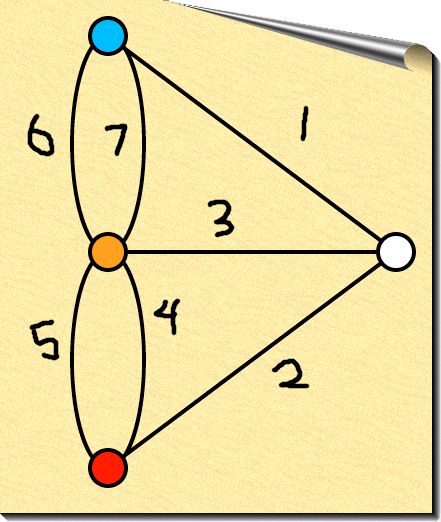
\includegraphics[scale=0.4]{bridge}}
\centerline{Labelled figure of the initial K\"onigsberg Bridge problem, taken from Wikipedia.} \\

Yes. If bridges 1 or 2 are demolished, then there is now a path so that the citizens can traverse the town, crossing every bridge exactly once and not end up where they started. \\

If bridge 1 is demolished, the path starting from Red is: \\

$5 \rightarrow 6 \rightarrow 7 \rightarrow 4 \rightarrow 2 \rightarrow 3$ ending at Orange. \\

If bridge 2 is demolished, the path starting from Blue is: \\

$6 \rightarrow 5 \rightarrow 4 \rightarrow 7 \rightarrow 1 \rightarrow 3$ ending at Orange.

\end{problem}

\begin{problem}
Show that a knight can tour each square on a $3\times 4$ chessboard -- though without finishing at the starting square. \\

\underline{Answer:} \\
Given a $3$x$4$ chessboard, we are able to divide the board into exactly $6$ black and $6$ white spaces. Using the same approach as we did in class, we are able to construct a bipartite graph. Using this graph, we can move the knight from a black space to a white space and vice versa, and as there are exactly $6$ black and white spaces, the knight can tour every square. \\

\centerline{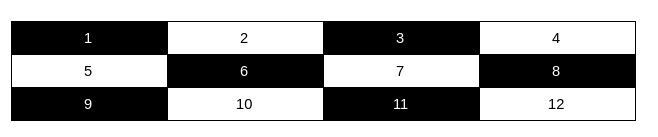
\includegraphics[scale=0.4]{chessboard.png}}
For this arrangement, the traversal is: \\

$1 \rightarrow 7 \rightarrow 9 \rightarrow 2 \rightarrow 8 \rightarrow 10 \rightarrow 3 \rightarrow 12 \rightarrow 6 \rightarrow 4 \rightarrow 11 \rightarrow 5$

\end{problem}

\begin{problem}
Write down the expression given by the parse tree.\\

\underline{Answer:} \\
(((4 * t) - (5 * w)) * (x + y)) * ((y + (w + z)) + (((2 * x) + 1 + y) + (5 * ($w^2$) + 3)))

\end{problem}

\begin{problem}
Consider a graph with five vertices and all $\binom{5}{2} = 10$ edges between the vertices. Color the edges red and blue so that there does not exist a monochromatic triangle. \\

\underline{Answer:} \\
\centerline{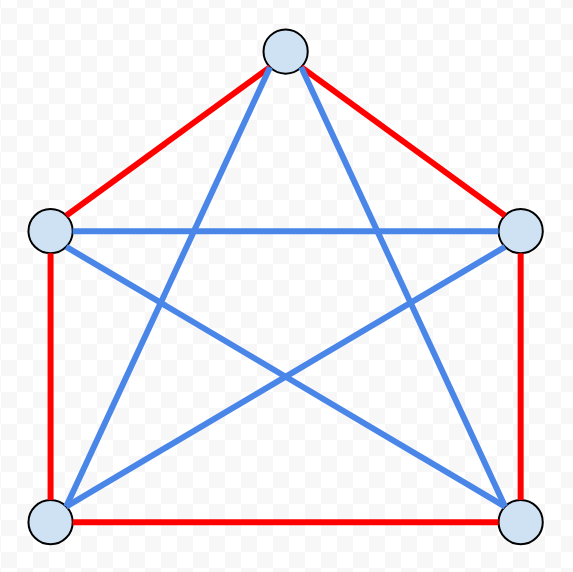
\includegraphics[scale=0.4]{q4.png}}

\end{problem}

\begin{problem}
In a party of 6 people is it true that  either there exists 4 people  who all do know each other or there exists 4 people who all do not know each other? Justify your answer. \\

\underline{Answer:} \\
\centerline{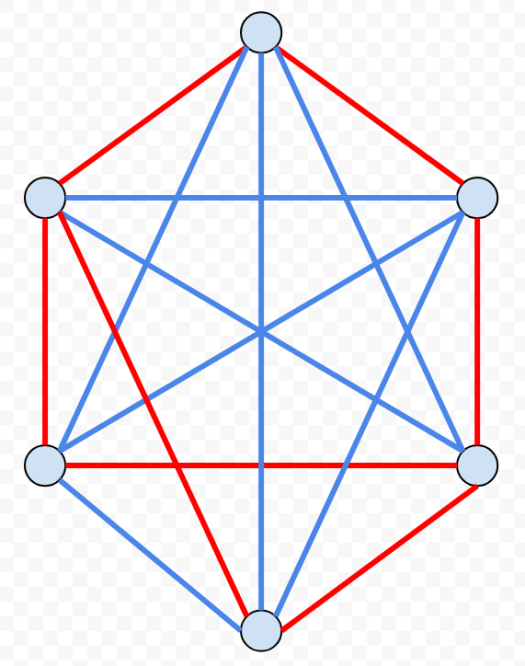
\includegraphics[scale=0.4]{q5.png}}

Another way to think of this is to look at Q4, in which we showed that for a graph with 5 vertices, there is a colouring such that there does not exist a monochromatic triangle. Thus, for a graph with 6 vertices, if we colour the edges correspondingly, there is a colouring such that there does not exist a monochromatic square. The figure above is simply one example of such a colouring.

\end{problem}

\begin{problem}
Prove that every (simple) graph with at least two vertices contains 2 vertices with the same degree. \\

\underline{Answer:} \\
Let G be a simple graph with $n$ vertices where $n \geq 2$. \\

Suppose that $G$ is a connected graph, then each vertex must have a degree from the set \{$1, n - 1\}$. As the graph has $n$ vertices, by the pigeon-hole principle, there must be two vertices that have the same degree. \\

Suppose that $G$ is not a connected graph, then each vertex cannot have a degree of $n - 1$ as that would be a connected graph. Thus, each vertex must have a degree from the set \{$0, n - 2\}$. As the graph has $n$ vertices, by the pigeon-hole principle, there must be two vertices that have the same degree.

\end{problem}

\end{document}
